\subsection{Self-healing - Auto-riparazione}
\begin{frame}\frametitle{Self-healing - Auto-riparazione}
    Il \emph{self-healing} è la capacità di un materiale di recuperare l'integrità a seguito di una frattura microscopica o macroscopica.
\begin{figure}{\centering{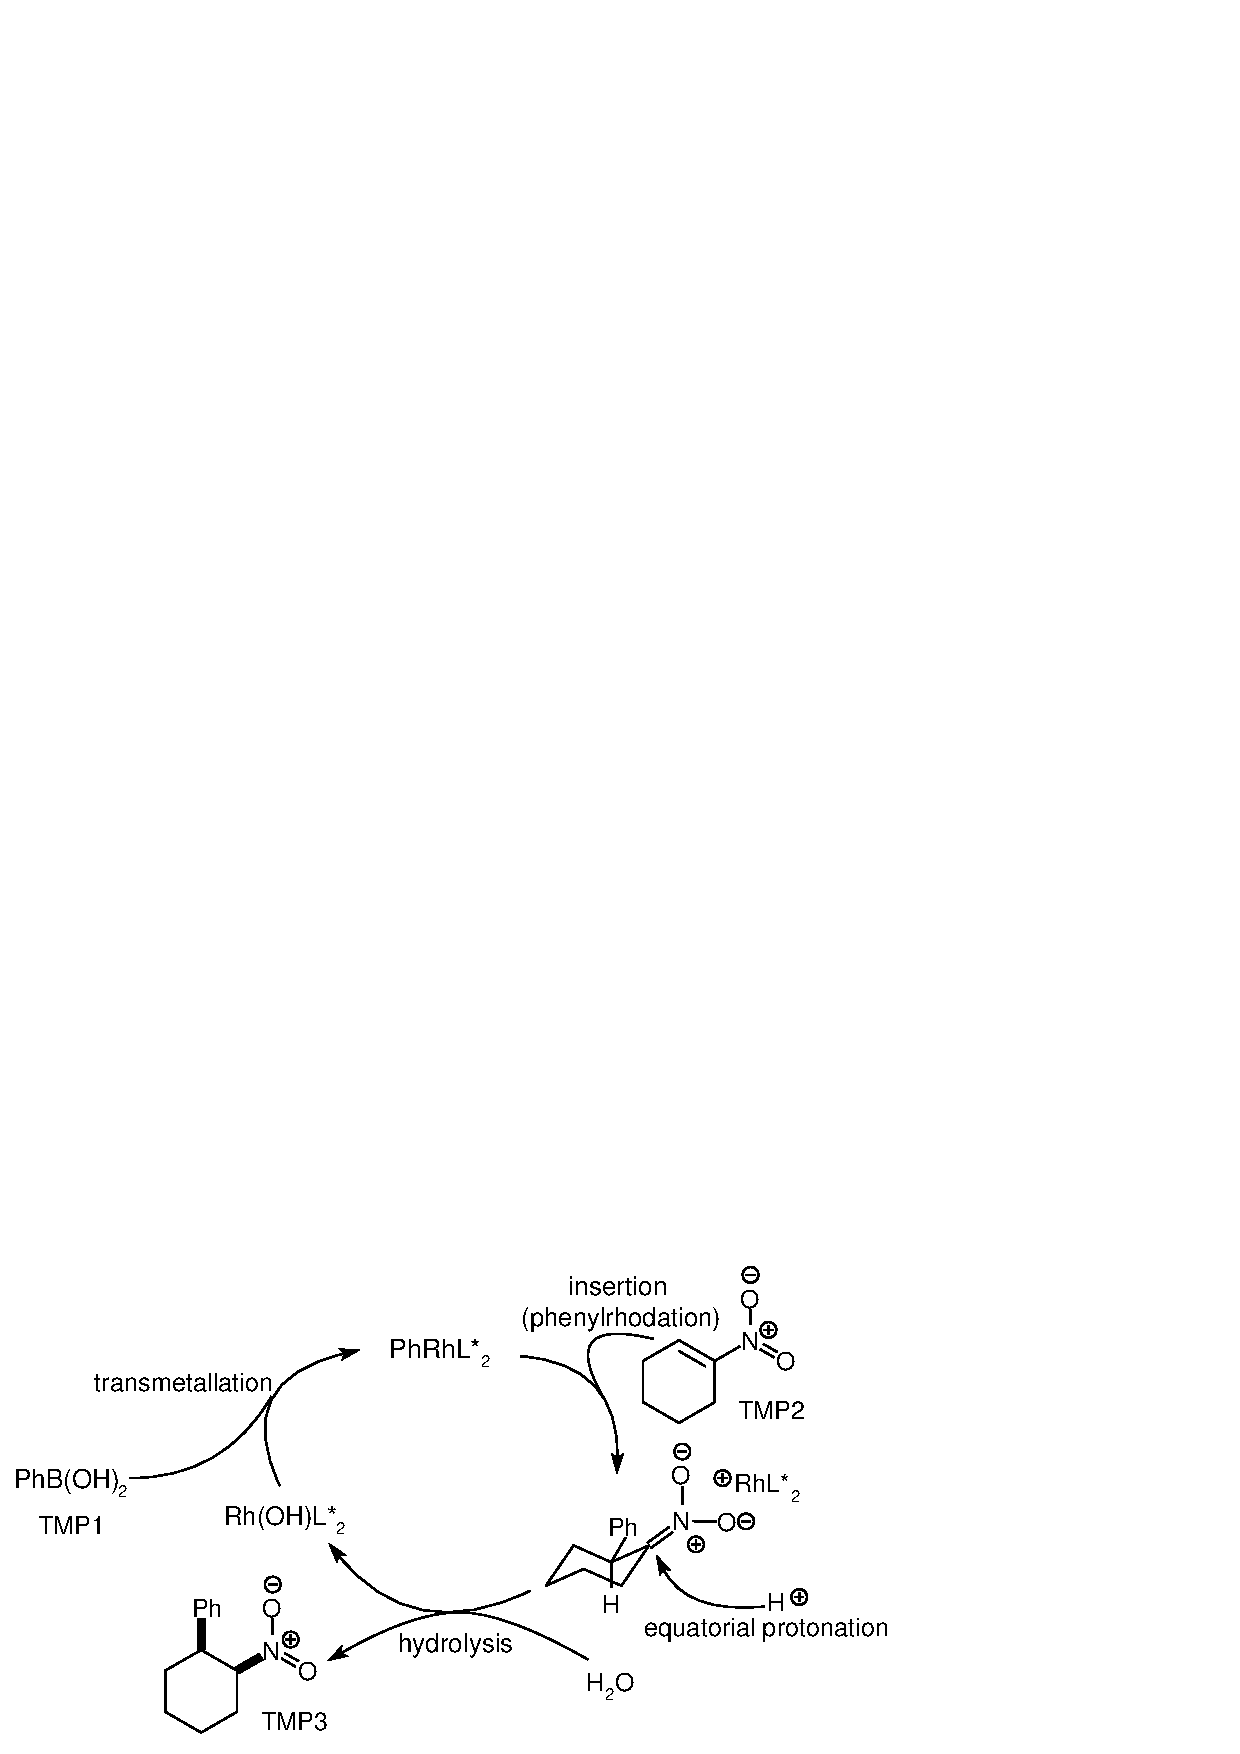
\includegraphics[width=0.7\textwidth]{intro/meccanismo.png}}}\end{figure}
{\small Principio di funzionamento. \\ a) Uno sforzo causa una frattura; b) si forma una ``fase mobile'';\\ c) la ``fase mobile'' chiude la frattura;
d) il tutto si blocca.}
\end{frame}

\subsection{Classificazioni del fenomeno}\begin{frame}\frametitle{Classificazioni del fenomeno}
I meccanismi di auto-riparazione possono essere classificati:
\begin{enumerate}
 \item \textbf{automatico}, la rottura è stimolo sufficiente alla riparazione;
 \item \textbf{non automatico}, richiede calore o luce;
\end{enumerate}

\begin{enumerate}
 \item \textbf{intrinseco}, il materiale di per sé è capace di ripararsi;
 \item \textbf{estrinseco}, è necessario inglobare materiali estranei; 
\end{enumerate}

\begin{enumerate}
 \item \textbf{reversibile}, nello stesso punto può ripararsi più volte;
 \item \textbf{irreversibile}.
\end{enumerate}
\end{frame}


\subsection{Materiali}\begin{frame}\frametitle{Materiali}
    Molti materiali possono essere realizzati la proprietà di \emph{self-healing}:
\begin{itemize}
 \item ceramica (produzione di massa ossidata alla frattura);\pause
 \item cemento (piccola frazione non idratata o \ce{CaCO3} formato da batteri);\pause
 \item acciai (sovrasaturando con B e N o con Cu) e leghe di alluminio;\pause
 \item \textbf{polimeri e polimeri supramolecolari}.
\end{itemize}

\footnote{\tiny  \fullcite{materiali}}



\end{frame}




\subsection{Polimeri tradizionali}\begin{frame}\frametitle{Polimeri tradizionali}
La \textbf{reticolazione} nei polimeri ne \textbf{riduce la riciclabilità} e ne aumenta la \textbf{fragilità} (bassa resilienza).

In questa presentazione verranno presentate strategie per arrivare ad una \textbf{riparazione} dell'inevitabile \textbf{danneggiamento} ed a un facile riciclo per de-polimerizzazione o de-reticolazione.

\vspace{10pt}

Utilizzando diversi approcci sono stati realizzati materiali plastici con la \textbf{capacità di riparare fratture} di dimensione microscopica o macroscopica \textbf{ponendo in contatto le superfici} di rottura.

\vspace{10pt}

In un materiale reticolato anche una rottura a livello macroscopico consiste in una \textbf{rottura a livello molecolare}, solitamente non riparabile.

\end{frame}
